\documentclass[tikz,border=7pt]{standalone}
\usepackage[scaled=0.95]{helvet}
\renewcommand{\familydefault}{\sfdefault}
\usepackage[europeanresistors,americanvoltages]{circuitikz}
\definecolor{TEJNavy}{HTML}{1E2B55}
\definecolor{TEJBlue}{HTML}{1769AA}
\begin{document}
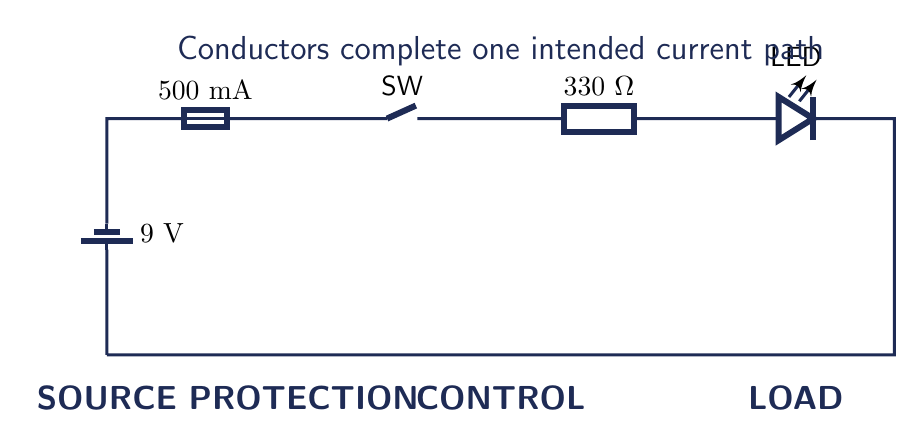
\begin{tikzpicture}[line width=1.1pt,draw=TEJNavy]
  \ctikzset{bipoles/length=1.1cm}
  \draw (0,0) to[battery1,l_=$9\ \mathrm{V}$] (0,3)
    to[fuse,l=$500\ \mathrm{mA}$] (2.5,3)
    to[nos,l=SW] (5.0,3)
    to[R,l=$330\ \Omega$] (7.5,3)
    to[leD,l=LED] (10.0,3) -- (10.0,0) -- (0,0);
  \node[font=\bfseries\large,text=TEJNavy] at (0,-0.55) {SOURCE};
  \node[font=\bfseries\large,text=TEJNavy] at (2.5,-0.55) {PROTECTION};
  \node[font=\bfseries\large,text=TEJNavy] at (5.0,-0.55) {CONTROL};
  \node[font=\bfseries\large,text=TEJNavy] at (8.75,-0.55) {LOAD};
  \node[font=\large,text=TEJNavy] at (5.0,3.85) {Conductors complete one intended current path};
\end{tikzpicture}
\end{document}
